\documentclass[conference]{IEEEtran}
\IEEEoverridecommandlockouts
% The preceding line is only needed to identify funding in the first footnote. If that is unneeded, please comment it out.
\usepackage{caption}
\usepackage{cite}
\usepackage{amsmath,amssymb,amsfonts}
\usepackage{algorithmic}
\usepackage{graphicx}
\usepackage{textcomp}
\usepackage{xcolor}
% User packages
\usepackage{hyperref}
\usepackage{makecell}

\renewcommand\theadalign{bc}
\renewcommand\theadfont{\bfseries}
\renewcommand\theadgape{\Gape[4pt]}
\renewcommand\cellgape{\Gape[4pt]}

% \usepackage[brazilian]{babel}

% Default arameters
\def\BibTeX{{\rm B\kern-.05em{\sc i\kern-.025em b}\kern-.08em
    T\kern-.1667em\lower.7ex\hbox{E}\kern-.125emX}}

% User parameters
\newcommand{\reviewUrgent}[1]{{\color{red} #1}} % This command is used for mandatory changes
\newcommand{\reviewNormal}[1]{{\color{yellow} #1}} % This command is used for a strong suggestion
\newcommand{\reviewMinor}[1]{{\color{green} #1}} % This command is used for minor changes suggestion

\begin{document}

\title{Dimensionality Reduction Analysis Applied to Breast Cancer Data}

\author{\IEEEauthorblockN{Brewton Morais}
\IEEEauthorblockA{\textit{DETI} \\
\textit{Universidade Federal do Ceará}\\
Fortaleza, Brazil \\
\href{mailto:brewtonlmorais@gmail.com}{brewtonlmorais@gmail.com}}
\and
\IEEEauthorblockN{Lucas Abdalah}
\IEEEauthorblockA{\textit{DETI} \\
\textit{Universidade Federal do Ceará}\\
Fortaleza, Brazil \\
\href{mailto:lucasabdalah@alu.ufc.br}{lucasabdalah@alu.ufc.br}}
}

\maketitle

\begin{abstract}
Breast Cancer is one of the most aggressive cancer types and has a great impact in cancer mortality, mainly in women. This work analyzes tumor cells characteristics in order to provide an effective method to preprocess and reduce the dimension of the data, since the presence of several predictors may provide redundant information, what increases the cost of a Machine Learning-based techniques. In this paper, we present a framework based in Principal Component Analysis (PCA) and data normalization to clean the data and extract only the more relevant parameters, that can preserve original data characteristics and feed a predicting model to provide a final diagnosis.

% Abstract: 104 words
% This document is a model and instructions for \LaTeX.
% This and the IEEEtran.cls file define the components of your paper [title, text, heads, etc.]. *CRITICAL: Do Not Use Symbols, Special Characters, Footnotes, 
% or Math in Paper Title or Abstract.
\end{abstract}

\begin{IEEEkeywords}
Breast Cancer, Dimensionality Reduction, Linear regression, Machine learning, Principal Component Analysis.
\end{IEEEkeywords}

\section{Introduction}
Breast Cancer is the most incident among women in the world and the leading cause of cancer death. In 2018, there were 2.1 million new cases, equivalent to 11.6\% of all cancers estimated. Regardless of the socioeconomic development of the country, the incidence of this cancer ranks among the top positions of female malignant neoplasms, even though the most frequent type of diagnosed cancer substantially vary across countries~\cite{Bray2018}.

After skin cancer, breast cancer is the most common cancer diagnosed in women in Brazil. Approximately 59,700 women were diagnosed in 2019, with a mortality rate of 13.68 per 100,000 habitants. There is not only one risk factor for breast cancer, however age over 50 is considered the most important~\cite{INCA2019}. Other factors that contribute to the increased risk of developing the disease are genetic factors and hereditary factors (cancer of ovary in the family), obesity, physical inactivity and exposure frequent exposure to ionizing radiation (environmental and behavioral factors)~\cite{Bray2018, INCA2019}.

The funding support for breast cancer has helped to emerge diagnosis and treatment advances. Survival rates have increased, and the number of deaths associated with the disease is declining, mainly due to factors such as earlier detection, better understanding of the disease and personalized approach~\cite{Rivera2018}. Some exams such as mammography and contrast-enhaced (CE) digital mammography are commonly used to do the diagnosis, as well as the breast biopses aims to infer if the tumor is malignant or benign, requiring trained people~\cite{Sledge2014, Cardoso2014}.

The main characteristics of malignant tumors, that causes various types of cancer, may be used as machine learning models input to assist in clinical diagnosis or even to provide an automated diagnosis. Retrieving tumor features such as texture, smoothness, radius size, etc. The stage of preprocessing and analysis of these parameters is crucial to the early-stage breast cancer detection~\cite{Street1993}. Various approaches exploiting the same dataset are available in literature, e.g, linear programming, machine learning, data mining, and optimization techniques~\cite{Bennett1992, Wolberg1994, Mangasarian1995}.

Throughtout this paper, the relevance of such cell caracteristics will be analyzed by statitics metrics and data visualization tools 
aiming to find correlation with the diagnosis. The main goal is build framework capable to provide preprocessed data to use in a probabilistic model able to predict the malignancy of tumor cells. These steps precede more complex analysis such as feature extraction, dimensionality reduction, clustering and class separation~\cite{Hastie2009, Kuhn2013, James2013}.

Futhermore, the Principal Component Analysis (PCA), is applied on the search for relationship between the parameters and their class, that may be categorized as a binary classification problem~\cite{Abdi2010}. The PCA is a celebrated method to compute predictors relationship and reduce the data dimension, and in this work we present the most relevant characteristics related to the malignant, based on the provided set.

\section{Methods}
\subsection{Data set overview}

The breast cancer is characterized when the cells in the women's breast start growing uncontrollaby, forming tumors that can be either bening or malign. The diagnosis predictor is the categorical variable, which it can be either \textbf{M} for Malignant, or \textbf{B} for Benign~\cite{Street1993}.

The dataset contains cell parameters such as radius mean, texture mean, area mean, smoothness and so on, which are normally the parameters altered by a malignant tumor. It is composed by 32 columns and 569 rows, i.e, 32 features for 569 samples. There are 2 columns between the 32 that do not represent any information concerning the cells, but the identification of the pacients and their final diagnosis as well. 

Although there are only two classes, the key challenge is to build a prediction model based on the weight of each feature on the final result, that is, the relevance on the final diagnosis. It's proposed a data investigation on the possible missing values as well as a dimensionality reduction by performing a PCA, since there are too many columns, what would make the model too complex and probably not able 
to generalize if all of these features were to be considered for the model construction. 

Throughout this work, the programming language \textit{\textbf{Python}} was employed 
using mainly the \textit{Pandas} library, which deals with data frame, including the 
preprocessing and cleaning steps, as well as the plots and inferences. 

As it was previously stated, the data set contains 32 columns whose 30 of them 
correspond to the predictors. The following list corresponds to the set of all 
variables present in the data frame and their definition, with order of appearance. 

\begin{table}[htbp]
\caption{Summary of Predictors Information.}
\begin{center}
\begin{tabular}{|c|c|}
    \hline
    \cline{2-2} 
    \textbf{Tag} & \textbf{Description} \\
    \hline
    id & Patient identification \\
    \hline
    Diagnosis & Sample class \\
    \hline
    Radius Mean & \makecell{Mean value of \\ lobes' radius} \\
    \hline
    Texture Mean & \makecell{Mean value of \\ surface texture} \\
    \hline
    Perimeter Mean & \makecell{Mean value of lobes' \\ outer perimeter} \\
    \hline
    Area Mean & \makecell{Mean value of \\ lobes' area} \\
    \hline
    Smoothness Mean & \makecell{Mean value of \\ smoothness level} \\
    \hline
    Compactness Mean & \makecell{Mean value of \\ tumor cell compactness} \\
    \hline
    Concavity Mean & \makecell{Mean value of tumor \\ cell concavity} \\
    \hline
    Concave Points Mean &  \makecell{Mean value of tumor\\ cell concave points} \\
    \hline
    Symmetry Mean & \makecell{Mean value of tumor\\ cell symmetry} \\
    \hline
    \makecell{Fractal \\ Dimension Mean} & \makecell{Mean value of tumor \\ cell fractal dimension} \\
    \hline
    Radius SE & Error of radius \\
    \hline
    Texture SE & Error of texture \\
    \hline
    Perimeter SE & Error of perimeter. \\
    \hline
    Area SE & Error of area \\
    \hline
    Smoothness SE & Error of smoothness \\
    \hline
    Compactness SE & Error of compactness \\
    \hline
    Concavity SE & Error of concavity \\
    \hline
    Concave Points SE & Error of concave points \\
    \hline
    Symmetry SE & Error of symmetry \\
    \hline
    Fractal Dimension SE & Error of fractal dimension \\
    \hline
    Radius Worst & Worst tumor cell radius value \\
    \hline
    Texture Worst & Worst tumor cell texture value \\
    \hline
    Perimeter Worst &  Worst tumor cell perimeter value\\
    \hline
    Area Worst &  Worst tumor cell area value \\
    \hline
    Smoothness Worst & Worst tumor cell smoothness value \\
    \hline
    Compactness Worst &  Worst tumor cell compactness value \\
    \hline
    Concavity Worst & Worst tumor cell compactness value \\
    \hline
    \makecell{Concave \\ Points Worst} & Worst concave points value \\
    \hline
    Symmetry Worst & Worst tumor cell symmetry value \\
    \hline
    \makecell{Fractal \\ Dimension Worst} & Worst tumor cell fractal value \\
    \hline
\end{tabular}
\label{tab:Summary}
\end{center}
\end{table}

\section{Data Preprocessing}
Before dealing with plots and inferences from the data, it is extremely important to 
perform a normalization in order to facilitate the visualization of the histograms 
and correlation plots. It is done by applying the z-score on the dataset.

\subsection{Z-Score Normalization}

Also called a standard score, the z-score is a normalization technique that gives the 
idea of how far from the mean a data point is. It can be placed on a 
\textit{normal distribution} curve. In order to do so, it is necessary to know the 
mean $\mu$ and the standard deviation $\sigma$ of the points.

Let $\Bar{x}$ be the sample mean,
$$\Bar{x} = \sum_i \frac{x_i}{N}$$
then
$$z_i = \cfrac{x_i - \Bar{x}}{\sigma}$$

Therefore, since now the data is located around a zero mean normal distribution with 
unitary variance, the identification of outliers has became easier.

The need to perform such normalization is that a model constructed from a 
non-normalized data set will probably have a biased result, since the model can be 
sensitive to variance. Thus, in a non-normalized data set, if there are large 
differences between the range of some variables, those with the highest range would 
have much more relevance to the model, since the variance is larger, that is, 

it carries more information.

\subsection{Data cleaning}\label{AA}
It was checked if there were any missing values, but it was found that all data is fully completed, 
which eliminates the need of any data compensation technique.

However, the first column containing the \textit{id} of the patients is not relevant for the analysis, so it's discarded during the analysis.

\clearpage

\subsection{Statistical Analysis}

Aiming to present a general perspective of the dataset, using the method \textit{describe} from the Pandas library, the table~\ref{tab:Data-Statistics} is a cutout of the entire table involving all parameters, here not shown in order to not difficult the comprehension.

The following table shows the mean statistics of 3 predictors grouped by 
Diagnosis: malignant or benign.

\begin{table}[htbp]
\caption{Data Statistics grouped by diagnosis.}
\begin{center}
\begin{tabular}{|c|c|c|c|}
    \hline
    \cline{2-4} 
    \textbf{Diagnosis} & \textbf{\textit{radius mean}}& \textbf{\textit{texture mean}}& \textbf{\textit{perimeter mean}} \\
    \hline
    \textbf{\textit{B}}& 1.097064 &-2.073335 &	1.269934  \\
    \hline
    \textbf{\textit{M}}& 1.829821 & -0.353632 & 1.685955 \\
    \hline
\end{tabular}
\label{tab:Statistics-by-diagnosis}
\end{center}
\end{table}

As it's possible to see in Fig.~\ref{fig:3-1-conditional-histogram}, the majority of variables present normal and exponential distribution. For the most part of the worst values for all the variables, it's not 
possible to infer a distribution density difference between then, since their values 
are really close to one another. Therefore, these variables are probably not 
informative for the final prediction. However, for values of radius mean, perimeter 
mean, area mean and smoothness mean, the difference is clear, indicating that 
those variables may have more relevance. 

Besides, some of the predictors, such as concave points mean and symmetry mean have 
similar distributions, which indicates a linear relationship between then. The same 
is found analysing the following columns of errors: radius, texture, perimeter, 
smoothness and compactness.

The linear relantionship between these predictors will be analysed using the pair 
plot soon.

% \clearpage
\subsection{Covariance Matrix and Predictors Relationship}

The degree of the linear relationship between two variables may be measured using the covariance coefficients $(p)$. It ranges from -1 to +1, where large positive and negative values indicates positively and negatively correlated data,respectively. Its absolute magnitude measures the degree of redundancy. If the covariance is close to zero, the data is uncorrelated~\cite{Kuhn2013}.

\begin{figure}[htbp!]
    \centerline{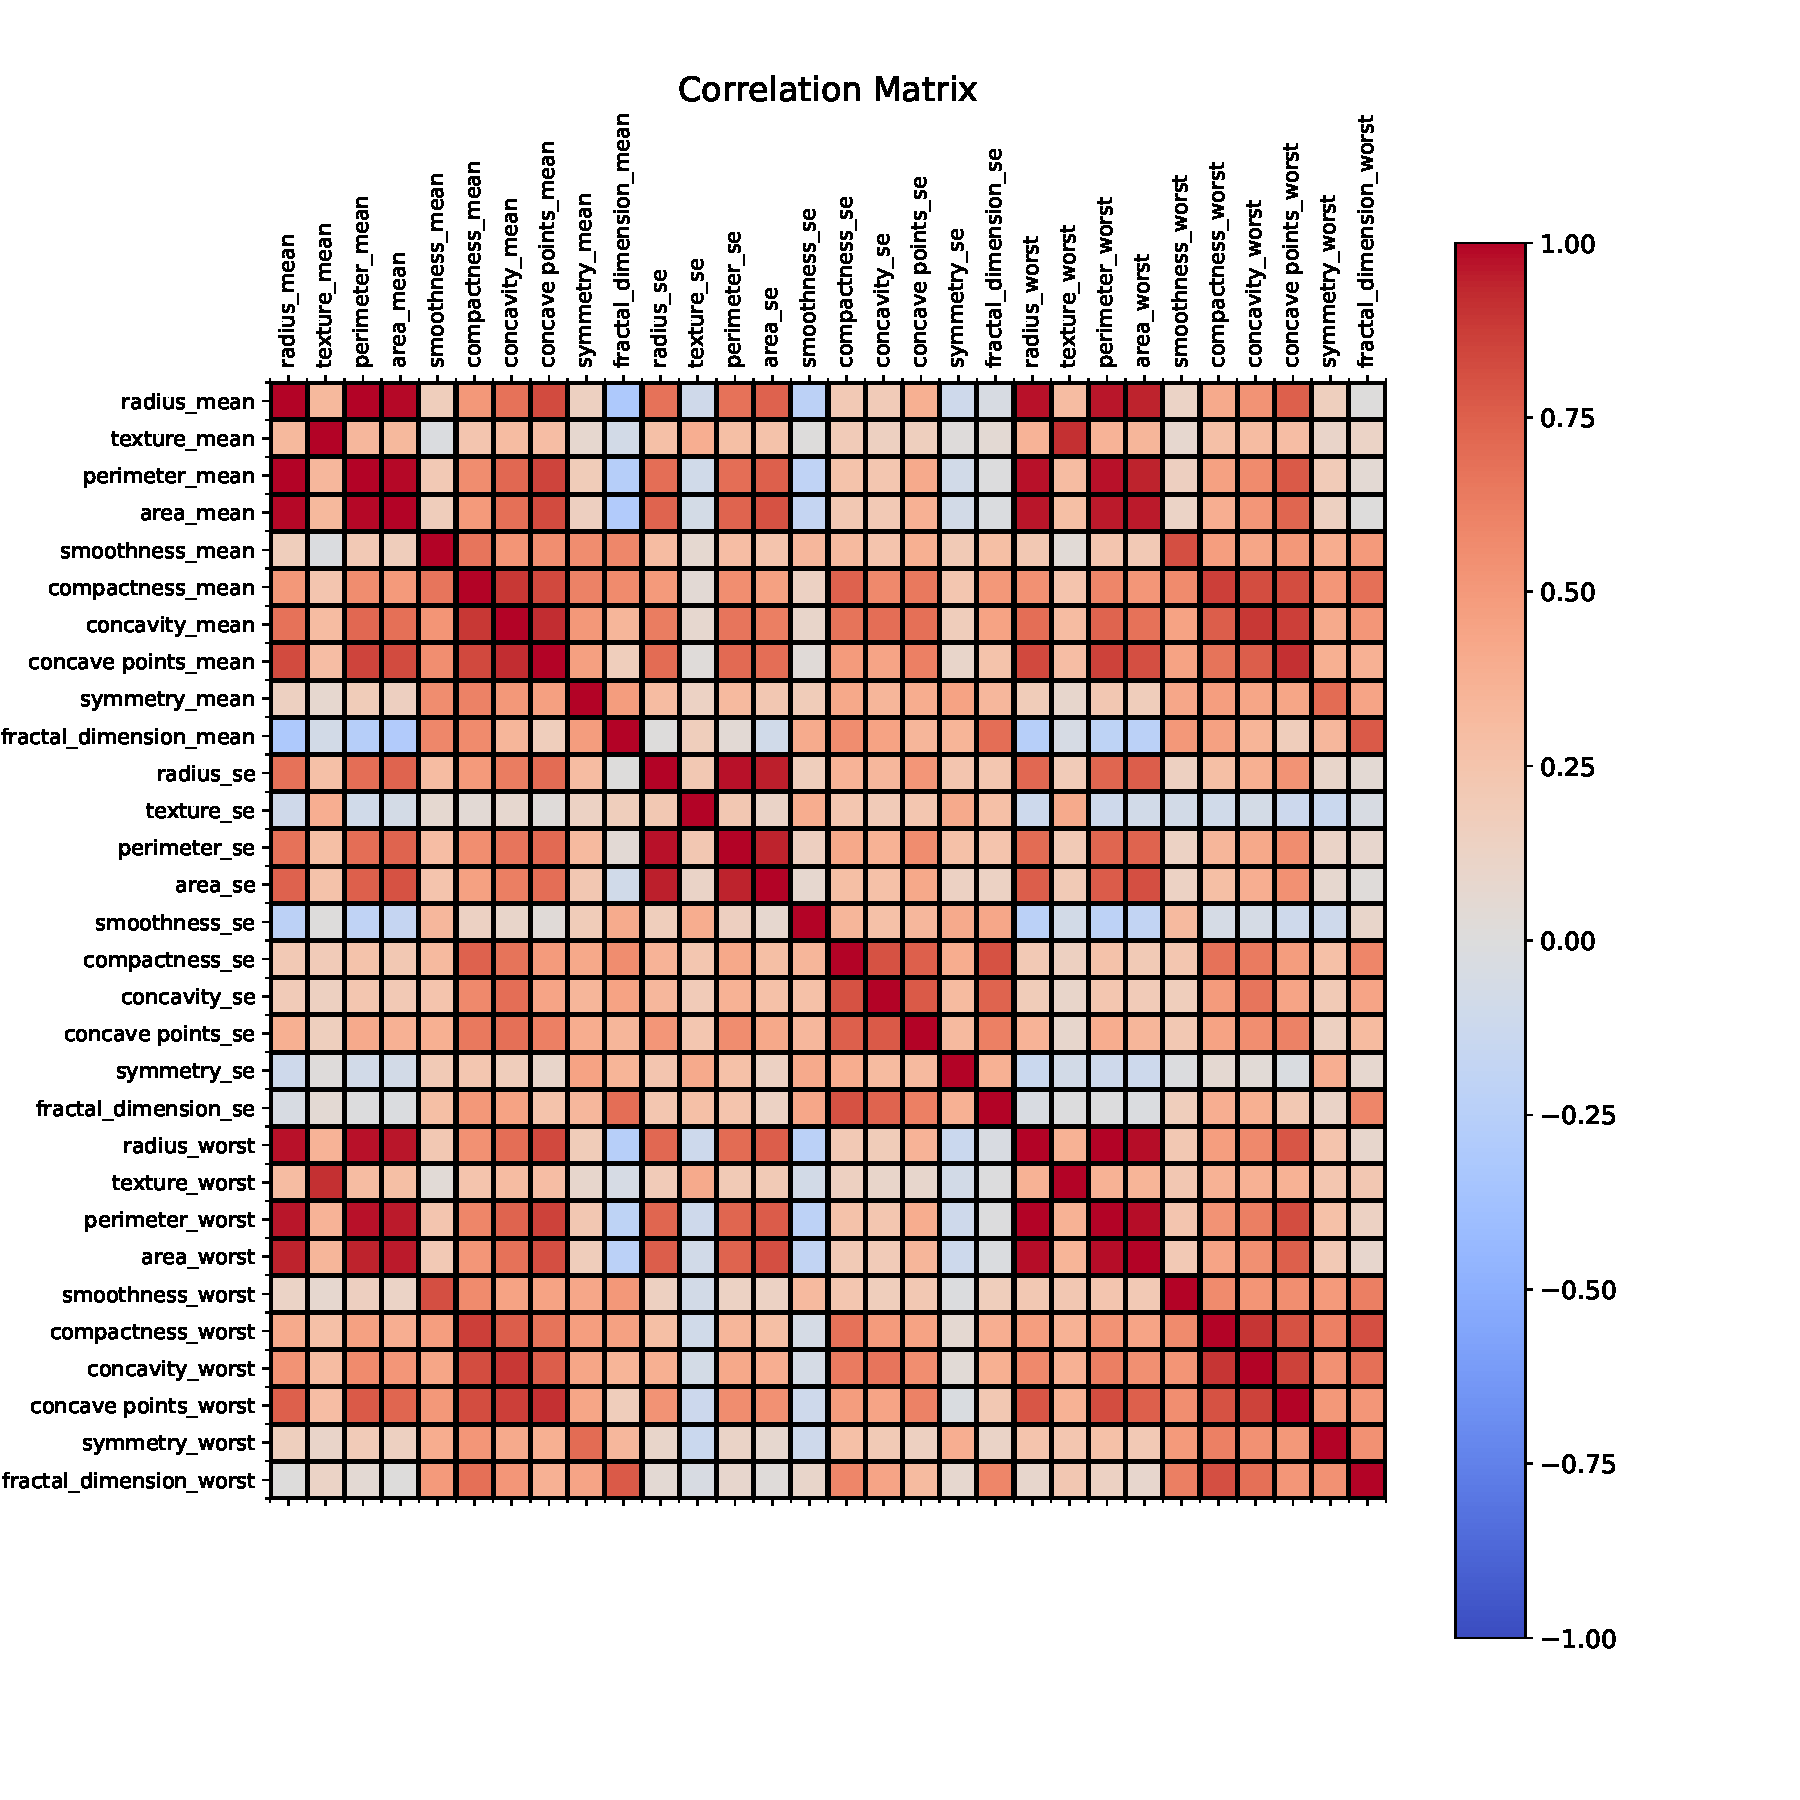
\includegraphics[width=0.5 \textwidth]{../../code/hw1/figures/4-3-correlation.pdf}}
    \caption{Correlation Matrix presented as a Heatmap.}
    \label{fig:4-3-correlation}
\end{figure}

In order to provide data covariance, we compute the covariance matrix and present it is a heatmap for visualization simplicity. Fig.~\ref{fig:4-3-correlation} shows that various predictors are strongly correlated, mainly positive.

\begin{table}[htbp]
\caption{Covariance threshold analysis.}
\begin{center}
\begin{tabular}{|c|c|}
        \hline 
        $|p| \geq$ & Related Pairs\\
        \hline
        $0.9$ & 21\\
        \hline
        $0.95$ & 15 \\
        \hline
\end{tabular}
\label{tab:Covariance}
\end{center}
\end{table}

For deepen the analysis, we use threshold two values for $|p|$ to assess how correlated data values, as shown in table~\ref{tab:Covariance}. 21 predictors pairs present a correlation coefficients $|p| > 0.9$, and 15 present a correlation coefficients $|p| > 0.95$.

\begin{figure}[htbp!]
    \centerline{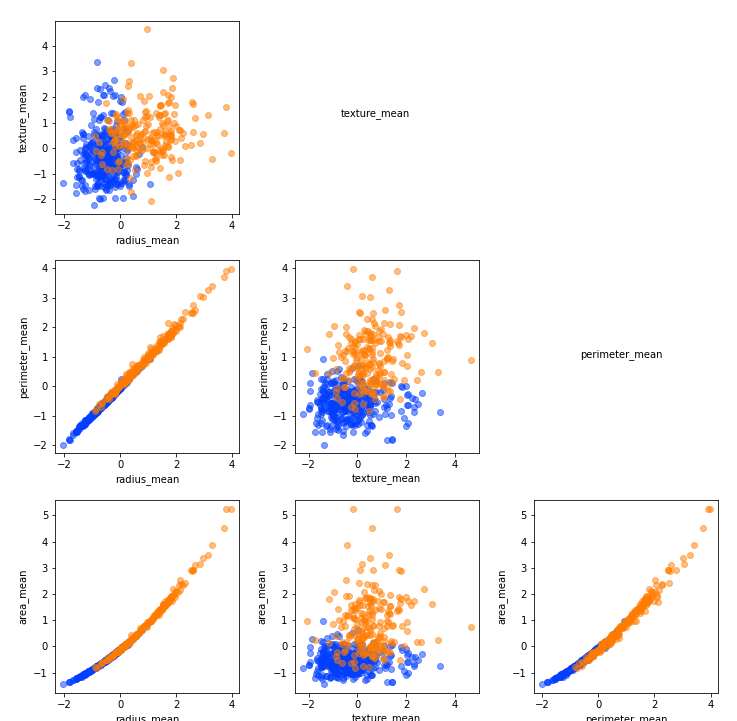
\includegraphics[width=0.5 \textwidth]{../../code/hw1/figures/4-1-scatter-plot-clip.png}}
    \caption{Scatter Plot.}
    \label{fig:4-1-scatter-plot}
\end{figure}

The covariance evidence combined with scatter plot analysis in Figure~\ref{fig:4-1-scatter-plot} provide more information to corroborate that our data carries a lot of redundancy. We can observe that the pair plots: Radius Mean vs. Perimeter Mean, Radius Mean vs. Area Mean and Perimeter Mean vs. Area Mean, present a linear behavior or very close to it.

% \clearpage

\subsection{Principal Component Analysis (PCA)}

PCA is a dimensionality reduction techninque that works by transforming a large set of variables into a smaller one that aims to represent as much as possible it's done by all the data variables. The justification for its implementation is that, at most part of the cases, it is worth losing a little accuracy in order to make a smaller data set. Besides, with a more compact data frame, it's less expansive to construct a machine learning model, because it'll work faster and the analysis will be easier. Thus, the goal is to preserve as much information as possible even after having performed the dimensionality-reduction.

\begin{figure}[htbp]
    \centerline{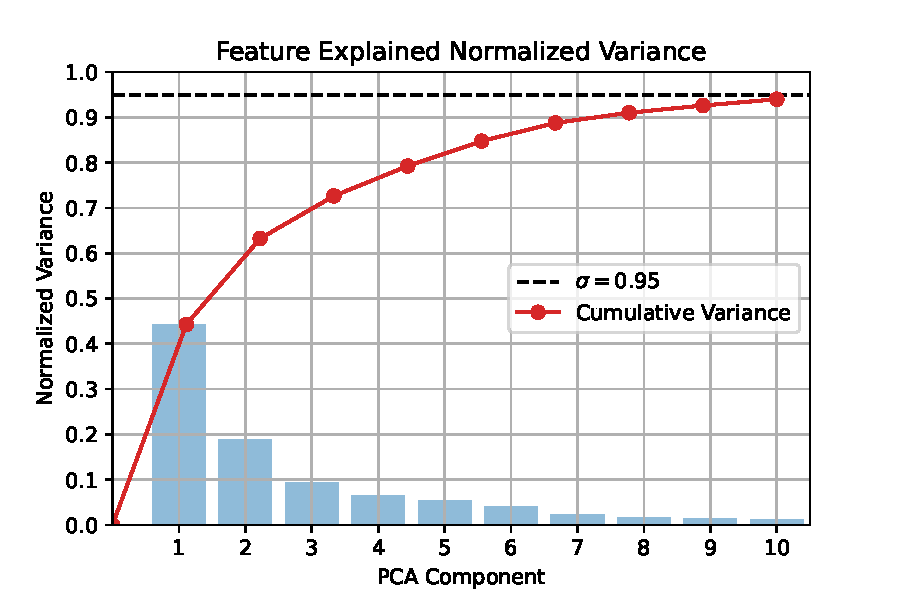
\includegraphics[width=0.5 \textwidth]{../../code/hw1/figures/5-1-PCA-10PC-variance.pdf}}
    \caption{Normalized Bar plot.}
    \label{fig:5-1-PCA-10PC-variance}
\end{figure}

We can see in Fig.~\ref{fig:5-1-PCA-10PC-variance}, the normalized variance, i.e, relevance on our context vs. the first 10 principal components (PC). We also present a cumulative curve, which shows that the first 2 PC carries more than 60\% of the variance, leading to 95\% with 10 PC, what we can interprete as only 10 columns of this dataset preserve 95\% from the original information. It means dividing the complexity by 3 and improving the storage and processing cost.

The PCA is a variance sensitive method, which won't be an issue, since all the columns were standardized with the \textit{Z-Score} application. 

The next stage is to compute the eigenvectors and its eigenvalues of the covariance matrix in order to identify the principal components. But first, the definition of Principal Components~\cite{Ringner2001}: principal components are directions along which the variance of the data reaches its maximal value. They are linear combinations of the initial variables, related in such a way that the new variables are uncorrelated and the most amount of information is present mainly within the initial components.

Since they are vectors, the principal components represent the directions of the data that explains a maximal variance, The fact that high variance indicates more 
information comes from the concept of entropy. 

Finally, the mathematics behind this algorithm for the first principal component consists in finding a line that maximizes the average of square distances from the points to the origin. Then, for the second component, it's done the same, but with the condition of being orthogonal to the first line found, since they must be uncorrelated. The process is the same for the remaining components. That's where the importance of eigenvectors and eigenvalues lies, the first represents the direction of the the axes where the variance is maximum and the latter the coefficients attached to it. 

As previously said, the first components always have more relevance, i.e, contain more information. Mathematically, once the eigenvectors are ordered according to their eigenvalues, the rank of principal components in significance is found as well.

Finally, from the eigenvectors a feature vector $(P)$ is created containing all of these eigenvectors or just some of them, after judging if some component is necessary or not, when they have less significance. 

\begin{equation}
    Y = P X
\end{equation}

So far, no data transformation was done apart from the normalization, so it's now necessary to recast the data along the principal component axes, which is done so by using the feature vector on the standardized data $(X)$ points in order to perform a reorientation.

\begin{figure}[htbp]
    \centerline{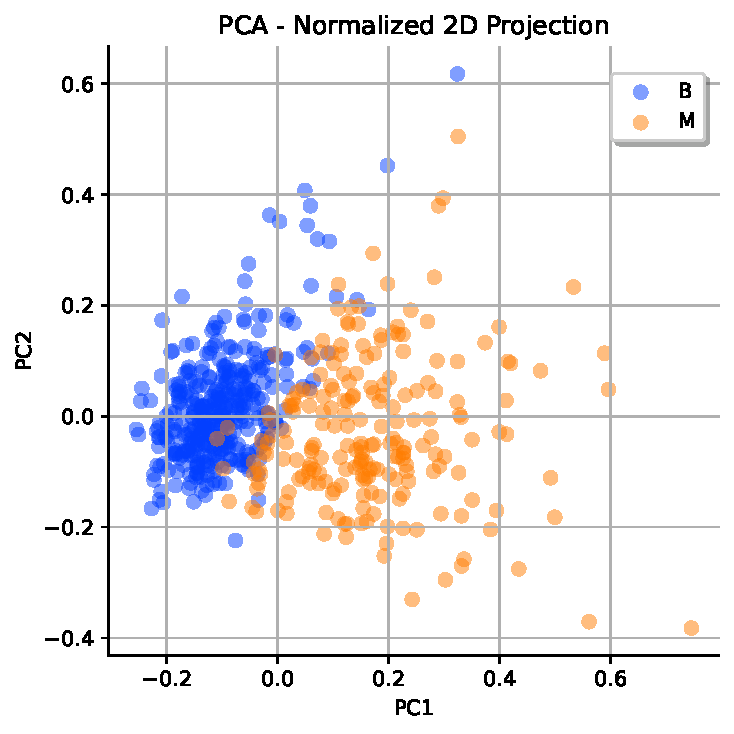
\includegraphics[width=0.5 \textwidth]{../../code/hw1/figures/5-2-PCA-2D-scatter.pdf}}
    \caption{Data scatter plot on the two principal components domain.}
    \label{fig:5-2-PCA-2D-scatter}
\end{figure}

After compute the projection, we can plot as shown in Fig.~\ref{fig:5-2-PCA-2D-scatter}, and observe that this component allow to split the data almost perfectly in two clusters.

\begin{figure}[htbp]
    \centerline{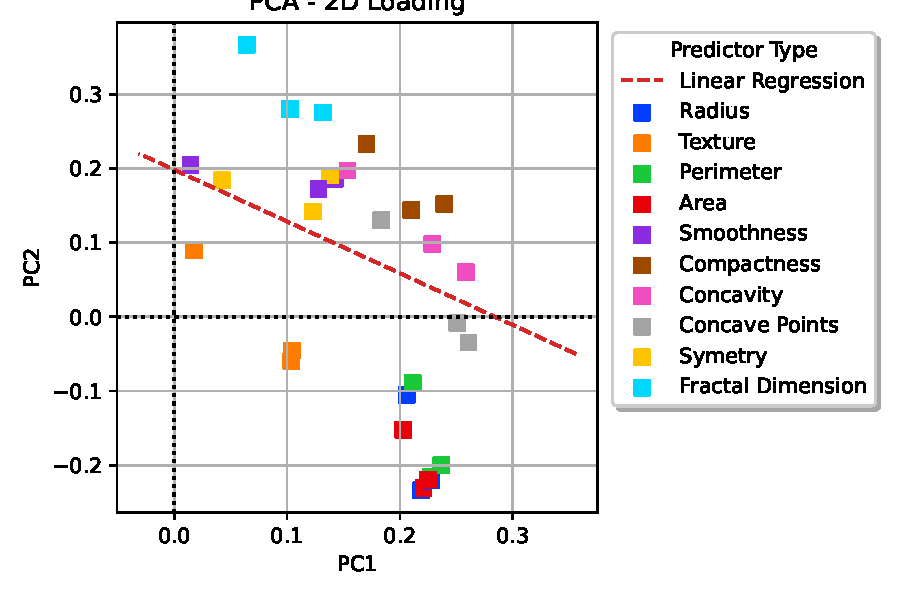
\includegraphics[width=0.5 \textwidth]{../../code/hw1/figures/5-2-PCA-2D-loading.pdf}}
    \caption{PCA loading with two principal components.}
    \label{fig:5-2-PCA-2D-loading}
\end{figure}

Fig.~\ref{fig:5-2-PCA-2D-loading} shows the loading, i.e, each predictor relevance on the projection variances of this 2 PC.

\section{Conclusion}

This work explored tatistical analyzes and the PCA application to visualize with clarity the behavioral patterns of the predictors in each class, in addition to the scatter trends, both being in a compact graphical representation. 

It is interesting to note that the dataset obtained at the end of this extraction of predictors represents the general idea (95\%) of the original dataset with only 10 PC. However, it is up to the modeler to decide whether this loss is offset by reduced computational complexity. It is worth mentioning that there are methods to further decrease the impact of predictor extraction of a dataset, although such methods have not been developed for the problem addressed here.

The use of the covariance matrix is to identify where it's possible to find redundant information, according to the correlation between a pair or variables. If the covariance between a pair of variables is highly positive, it means that they are correlated and the increase of one implies the increase of the other. For covariance between pairs being negative, they called inversely correlated, the increase of one implies the decrease of the other.

% \clearpage

\begin{table*}[htbp]
    \caption{Unconditional Data Statistics for the Mean Predictors}
    \begin{center}
        \begin{tabular}{|c|c|c|c|c|c|c|c|c|c|c|}
            \hline
            \cline{2-4} 
            & \textbf{\textit{radius}}& \textbf{\textit{texture}}& \textbf{\textit{perimeter}} & \textbf{\textit{area}} & \textbf{\textit{smoothness}} & \textbf{\textit{compactness}} & \textbf{\textit{concavity}} & \textbf{\textit{\makecell{concave \\ points}}} & \textbf{\textit{symmetry}} & \textbf{\textit{\makecell{fractal\\ dimension}}} \\
            \hline
            \textbf{\textit{count}}& 569 & 569 & 569  & 569  & 569 & 569  & 569 & 569 & 569  & 569  \\
            \hline
            \textbf{\textit{mean}}&  14.12 & 19.28 & 91.96 & 654.88 & 0.09 & 0.10 & 0.08 &0.04 & 0.18 & 0.06  \\
            \hline
            \textbf{\textit{std}}& 3.52 & 4.30 & 24.29 & 351.91 & 0.01 & 0.05 &0.07 & 0.03 & 0.02 & 0.00  \\ 
            \hline
            \textbf{\textit{skewness}} & 0.94 & 0.65 & 0.99 & 1.64 & 0.45 & 1.19 & 1.40 & 1.17 & 0.72 & 1.30  \\
            \hline
            \textbf{\textit{min}} &6.98	&9.71 & 43.79 & 143.50 & 0.05 & 0.01 & 0.00 & 0.00	& 0.10	& 0.04 \\ 
            \hline
            \textbf{\textit{25\%}}&11.70 & 16.17 & 75.17 & 420.30 & 0.08 & 0.06 & 0.02 & 0.02 & 	0.16 & 0.05 \\
            \hline
            \textbf{\textit{50\%}}& 13.37 &	18.84 & 86.24 & 551.10 & 0.09 &	0.09 & 0.06 & 	0.03 & 0.17 & 0.06 \\ 
            \hline
            \textbf{\textit{75\%}}& 15.78 & 21.80 & 104.10 & 782.70 & 0.10 & 0.13 & 0.13 &	0.07 & 0.19 & 0.06 \\ 
            \hline
            \textbf{\textit{max}}& 28.11 & 39.28 & 188.50 &	2501.00 & 0.16 & 0.34 & 0.42 &	0.20 & 0.30 & 0.09 \\ 
            \hline
    \end{tabular}
    \label{tab:Data-Statistics}
    \end{center}
    \end{table*}


\begin{figure*}[htpb!]
    \centerline{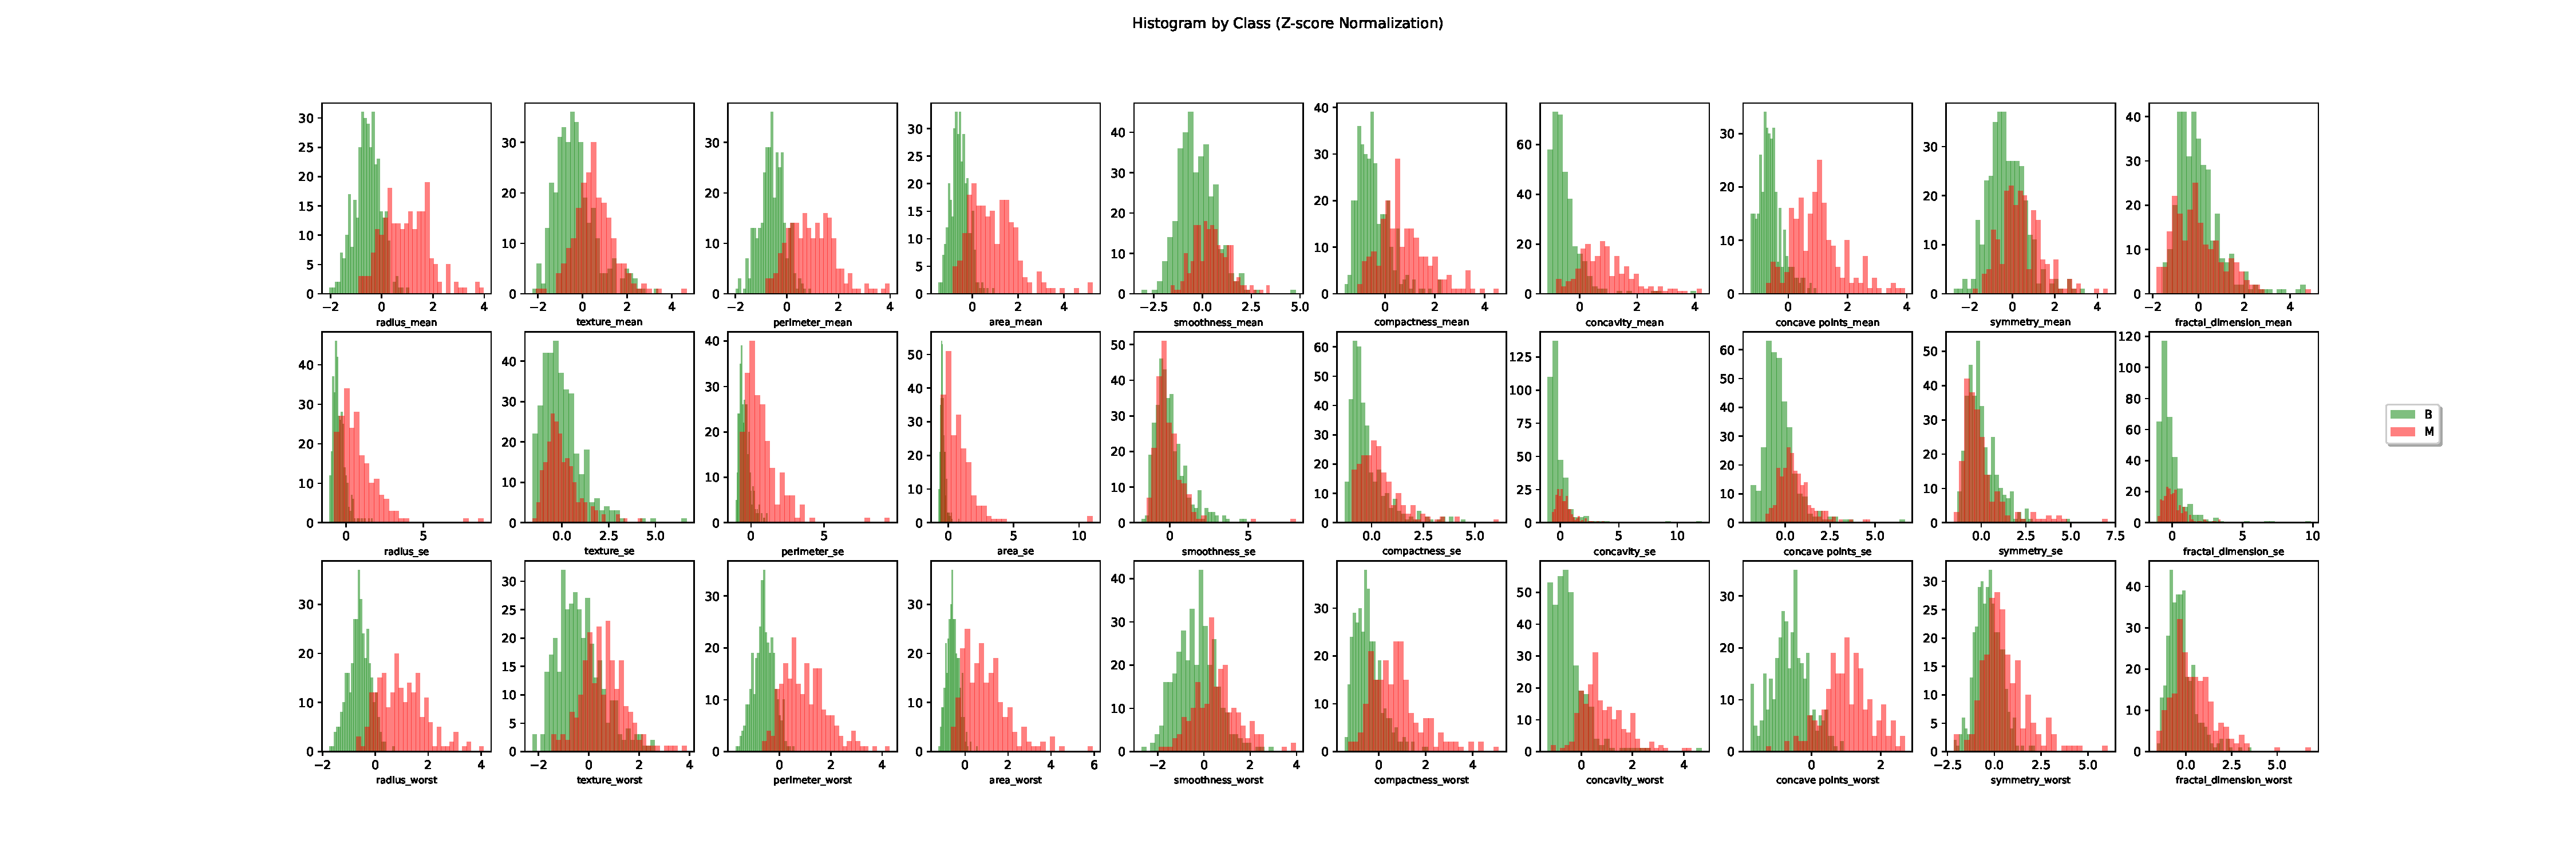
\includegraphics[width=1.2 \textwidth]{../../code/hw1/figures/3-1-conditional-histogram.pdf}}
    \caption{Conditional Histogram.}
    \label{fig:3-1-conditional-histogram}
\end{figure*}

% \clearpage
\bibliographystyle{ieeetran}
\bibliography{refs}


\end{document}
